\documentclass[12pt]{article}

\usepackage{float}

\usepackage{standalone}

\usepackage[utf8x]{inputenc}

%%% PAGE DIMENSIONS
\usepackage{geometry}
\geometry{a4paper}
\geometry{margin=2.54cm} % for example, change the margins to 2 inches all round

\usepackage{graphicx} % support the \includegraphics command and options

\usepackage[parfill]{parskip} % Activate to begin paragraphs with an empty line rather than an indent

%%% PACKAGES
\usepackage{booktabs} % for much better looking tables
\usepackage{array} % for better arrays (eg matrices) in maths
\usepackage{paralist} % very flexible & customisable lists (eg. enumerate/itemize, etc.)
\usepackage{verbatim} % adds environment for commenting out blocks of text & for better verbatim
\usepackage{subfig} % make it possible to include more than one captioned figure/table in a single float
% These packages are all incorporated in the memoir class to one degree or another...

\usepackage{multicol}
\usepackage{multirow}
\usepackage{xcolor}
\usepackage{amsmath}

\usepackage[T1]{fontenc}
\usepackage{lmodern}

\usepackage{makecell}

\renewcommand{\arraystretch}{1.1}

%%% HEADERS & FOOTERS
\usepackage{fancyhdr} % This should be set AFTER setting up the page geometry
\pagestyle{fancy} % options: empty , plain , fancy
\fancyhead[L]{\leftmark}
\fancyhead[C]{}
\fancyhead[R]{\rightmark}
\fancyfoot[L]{}
\fancyfoot[C]{}
\fancyfoot[R]{\thepage}
\renewcommand{\headrulewidth}{0pt}
\renewcommand{\footrulewidth}{0pt}

\fancypagestyle{plain}{
	\fancyhf{} % clear all header and footer fields
	\fancyfoot[R]{\thepage} % except the center
	\renewcommand{\headrulewidth}{0pt}
	\renewcommand{\footrulewidth}{0pt}
}

%%% BIBILIOGRAPHY
\usepackage[numbers]{natbib}
\bibliographystyle{vancouver}

%%% SECTION TITLE APPEARANCE
\usepackage{sectsty}
\allsectionsfont{\sffamily\mdseries\upshape} % (See the fntguide.pdf for font help)
% (This matches ConTeXt defaults)

%%% ToC (table of contents) APPEARANCE
\usepackage[nottoc,notlof,notlot]{tocbibind} % Put the bibliography in the ToC
\usepackage[titles,subfigure]{tocloft} % Alter the style of the Table of Contents
\renewcommand{\cftsecfont}{\rmfamily\mdseries\upshape}
\renewcommand{\cftsecpagefont}{\rmfamily\mdseries\upshape} % No bold!

\usepackage[bookmarks,bookmarksnumbered,bookmarksopen,hidelinks]{hyperref}

\usepackage{bookmark}


%%% TITLE
\title{Models for antibody data}
\author{Arseniy Khvorov, David Price, Annette Fox, Sheena G. Sullivan}
\begin{document}

%%% Title
\maketitle

%%% Main Contents

\subsection{The Kiddivax study}

The Kiddivax study was a randomized controlled trial undertaken in Hong Kong in 2009-2010 in which 796 children aged 6-17 years were randomized to receive inactivated vaccine. Blood samples were taken pre and 1 month post-vaccination to estimate their vaccine-induced antibody titres.  The children and their household contacts were followed for about 7 months for signs of influenza-like illness. Symptoms reported by any household member prompted swabbing and influenza testing by PCR for all household members \citep{Cowling;2013}. The protective titre could be estimated using a Cox proportional hazards model where the outcome was time to infection or the end of the study \citep{Ng;2013}.

%==============================================================================
\section{Kiddyvax application}

The data for this study includes post-vaccination HI titres of subjects who were followed for up to one year for flu infection. The infection status was determined by PCR which was done for everyone who experienced symptoms. This data is shown in Figure \ref{fig:kiddyvax-main-titre}.

\begin{figure}[htp]
	\centering
	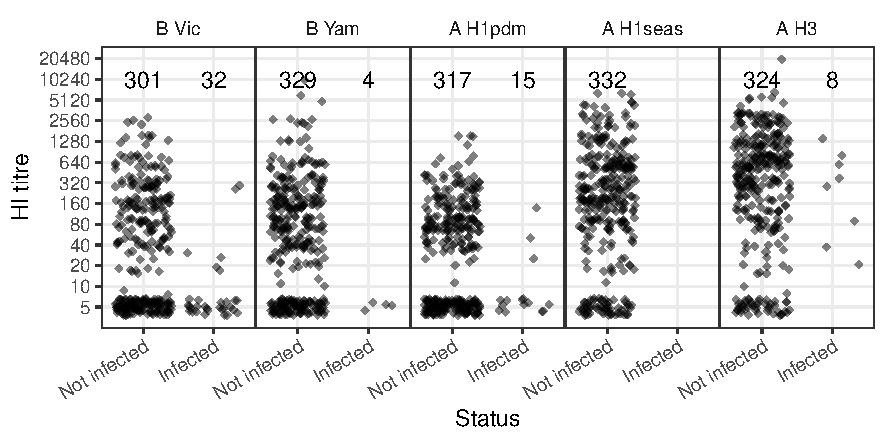
\includegraphics[width=1\textwidth]{../data-plot/kiddyvax-main-titre.pdf}
	\caption{
	Kiddyvax study data. Post-vaccination titres are shown for those who got infected (PCR-confirmed symptomatic infection) over the course of the study and those who did not. Panels correspond to the five tested viruses.
	}
	\label{fig:kiddyvax-main-titre}
\end{figure}

Analyses were done on the data for B Vic and A(H1pdm) viruses in the same way as for the Ha Nam data with the addition of the Cox proportional hazards model.

%\pagebreak
%
\subsection{Scaled logit fit}

The same scaled logit model was fit in the same way using the same prior distributions as for the Ha Nam data. The protection curves are in Figure \ref{fig:kiddyvaxmain-prot-bayes-sclr}. The credible intervals are very broad due to the fact there are very few infections the sample.

\begin{figure}[htp]
	\centering
	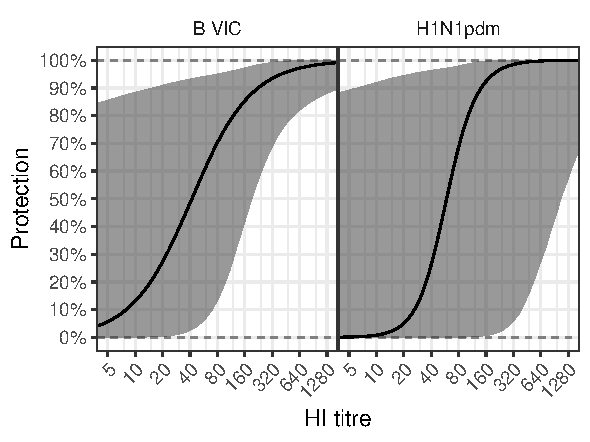
\includegraphics[width=0.8\textwidth]{../fit-sclr-bayesian-plot/kiddyvaxmain-prot.pdf}
	\caption{
Fitted infection curve and credible interval from the scaled logit model Bayesian fit to subsets of kiddyvax data (shown in Figure \ref{fig:kiddyvax-main-titre}). The solid line is the median of the posterior distribution. The shaded region is the 95\% credible interval. The dashed line is the prior distribution, i.e. the bounds of the shaded region that would have been obtained if the data contained no information to estimate model parameters.
	}
	\label{fig:kiddyvaxmain-prot-bayes-sclr}
\end{figure}



%\pagebreak
%
\subsection{Standard logistic fit}

The relative protection curves are in Figure \ref{fig:kiddyvaxmain-prot-rel-lr-boot}. The same considerations regarding the unjustified assumption of baseline risk of 1 apply here as they did with Ha Nam (Figure \ref{fig:kiddyvax-main-titre} shows many uninfected subjects with undetectable titres).

\begin{figure}[htp]
	\centering
	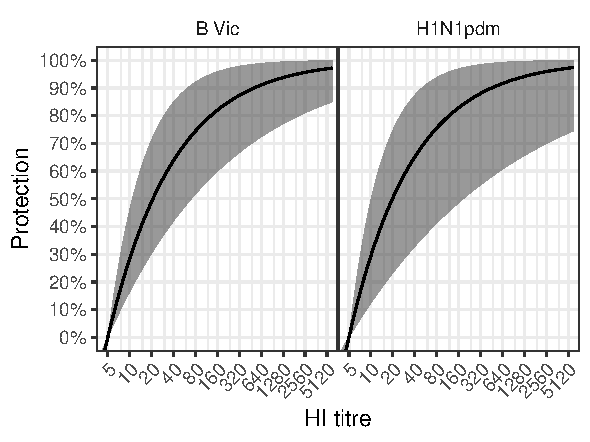
\includegraphics[width=0.8\textwidth]{../fit-logistic-boot-plot/kiddyvaxmain-prot-rel.pdf}
	\caption{
	Fitted relative-to-5 protection curves and confidence intervals from the standard logistic model fit to kiddyvax data (shown in Figure \ref{fig:kiddyvax-main-titre}) using maximum likelihood with no accounting of censored titres (observations of 5 (below detectable) were unchanged, all other observations were moved to the midpoints of the corresponding censored intervals on a log scale). The solid line is the point estimates. The shaded region is the 95\% confidence interval.
	}
	\label{fig:kiddyvaxmain-prot-rel-lr-boot}
\end{figure}

%\pagebreak
%------------------------------------------------------------------------------
\subsection{Cox proportional hazards fit}

For infected individuals, the time at risk was taken to be the time from start of follow-up to infection. For those who did not get infected the time at risk was take to be the time from start of follow-up to end of follow-up.

The model was

\begin{align*}
\begin{gathered}
h(t) = h_0\text{exp}(\beta_T X_{\text{logtitre}})
\end{gathered}
\end{align*}

where $h$ is the hazard function and $X_{\text{logtitre}}$ is the post-vaccination titre measurement on the log scale. The resulting protection curves (relative to the titre of 5) are in Figure \ref{fig:kiddyvaxmain-cox}. Although the point estimates are similar to those recovered from the model; however standard errors are inflated. 

\begin{figure}[htp]
	\centering
	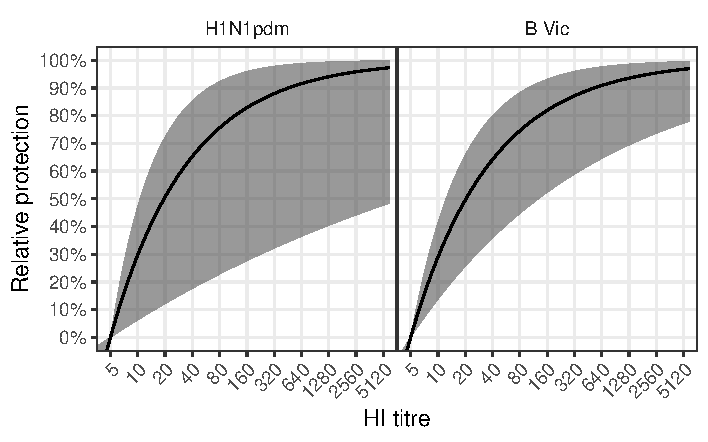
\includegraphics[width=0.8\textwidth]{../fit-cox-plot/kiddyvaxmain.pdf}
	\caption{
	Fitted relative-to-5 protection curves and confidence intervals from the Cox proportional hazards model fit to kiddyvax data (shown in Figure \ref{fig:kiddyvax-main-titre}) with no accounting of censored titres (observations of 5 (below detectable) were unchanged, all other observations were moved to the midpoints of the corresponding censored intervals on a log scale). The solid line is the point estimates. The shaded region is the 95\% confidence interval.
	}
	\label{fig:kiddyvaxmain-cox}
\end{figure}

\end{document}

